%
% Introduction
%

\chapterimage{Galileos-telescope-002.pdf} % Chapter heading image

\chapter{Introduction}
\label{chap:Introduction}

\begin{quote}
\begin{flushright}
\emph{If presented with a choice between indifferent alternatives,\\
then one ought to select the simplest one.}\\
Occam's razor principle 
\end{flushright}
\end{quote}
\bigskip

We live in an age where knowledge has become one of our most valued resources, driving economic progress and societal well-being. Science continually provides deeper insights into the world around us, leading to remarkable advances in fields ranging from medicine to digital technologies. Yet, despite this progress, our scientific understanding remains incomplete. We continue to encounter phenomena that we cannot adequately explain, questions that we cannot answer, and limitations that prevent us from fully understanding the entities we investigate.

A fundamental challenge arises from the way scientific knowledge is constructed. We study entities through representations, such as observations, measurements, and symbolic records, and develop descriptions or models to account for these representations. However, representations may omit essential information or contain irrelevant information, while descriptions may fail to capture the structure of their representations or introduce unnecessary complexity. These two sources of imperfection limit our understanding, even when our scientific methods are otherwise rigorous.

The \emph{theory of nescience} proposes a mathematical framework for studying these limitations and quantifying our lack of knowledge. By distinguishing between the inadequacy of representations, called \emph{miscoding}, and the inadequacy of descriptions, called \emph{mismodel}, the theory formulates scientific progress as the joint reduction of these two quantities. This volume develops the mathematical foundations of this approach, investigating the nature of scientific knowledge, the conditions for its improvement, the possibility of perfect knowledge, and the boundaries separating what is known from what remains unknown.

%
% Section: Scientific Knowledge
%

\section{Scientific Knowledge}

The pursuit of scientific knowledge begins with identifying the \emph{entities}\index{Entity} we seek to understand. These entities are extraordinarily diverse: mathematicians study abstract structures, biologists investigate living organisms, and engineers examine technological systems. Our quest for understanding is driven by the desire to explain phenomena, predict outcomes, and solve problems. For instance, we know that applying sufficient heat to wood will cause it to ignite, or that a fever may indicate an infection. Scientific understanding therefore depends on our ability to recognize patterns, identify regularities, and develop models that account for the entities under investigation.

However, scientific inquiry does not generally provide direct access to the entities we study. Instead, we construct \emph{representations}\index{Representation}, such as observations, measurements, texts, or datasets, that capture information about these entities. We then develop \emph{descriptions}\index{Description}, such as mathematical models or computational procedures, intended to account for these representations. Ideally, a representation would faithfully encode its entity, and a description would reconstruct that representation accurately and economically. Figure \ref{fig:representationProblem} illustrates this fundamental distinction: our descriptions do not reconstruct entities directly, but rather operate through their representations.

% A4
% \begin{figure}[t]
% \centering
% \begin{tikzpicture}
%     \node[draw, ellipse, minimum width=3cm] (entities) at (0,0) {Entities};
%     \node[draw, ellipse, minimum width=3cm] (representations) at (5,0) {Representations};
%     \node[draw, ellipse, minimum width=3cm] (descriptions) at (10,0) {Descriptions};
% 
%     \draw[-{Latex[length=3mm]}] (representations) -- node[above,midway] {encode} (entities);
%     \draw[-{Latex[length=3mm]}] (descriptions) -- node[above,midway] {model} (representations);
%     \draw[dashed,-{Latex[length=3mm]}] (descriptions) to [bend right=45] node[above,midway] {explain?} (entities);
% \end{tikzpicture}
% \caption{\label{fig:representationProblem}The Problem of Understanding}
% \end{figure}

% Octavo
\begin{figure}[t]
\centering
\begin{tikzpicture}
    \node[draw, ellipse, minimum width=1.5cm] (entities) at (0,0) {Entities};
    \node[draw, ellipse, minimum width=1.5cm] (representations) at (4.25,0) {Representations};
    \node[draw, ellipse, minimum width=1.5cm] (descriptions) at (9,0) {Descriptions};

    \draw[-{Latex[length=3mm]}] (representations) -- node[above,midway] {encode} (entities);
    \draw[-{Latex[length=3mm]}] (descriptions) -- node[above,midway] {model} (representations);
    \draw[dashed,-{Latex[length=3mm]}] (descriptions) to [bend right=45] node[above,midway] {explain?} (entities);
\end{tikzpicture}
\caption{\label{fig:representationProblem} The Problem of Understanding}
\end{figure}

This approach reveals two fundamental sources of imperfection in scientific knowledge. First, a representation may fail to encode an entity adequately, either because essential information is missing or because irrelevant information has been included. We call this inadequacy \emph{miscoding}\index{Miscoding}. Second, even when an adequate representation is available, its description may fail to reconstruct it correctly or may contain unnecessary complexity. We call this inadequacy \emph{mismodel}\index{Mismodel}.

Together, miscoding and mismodel characterize our lack of knowledge about an entity, which we call \emph{nescience}\index{Nescience}. Rather than combining these two components into a single measure, the theory treats nescience as a two-dimensional quantity, with miscoding and mismodel as distinct objectives to be minimized simultaneously. This provides a mathematical framework for evaluating scientific understanding, identifying its limitations, and studying how knowledge may be progressively improved through better representations and descriptions.

%
% Section: Entities
%

\section{Entities}

The theory of nescience begins by specifying the domain of entities about which knowledge is sought. Scientific inquiry is directed toward a wide variety of objects: planets, particles, languages, ecosystems, social institutions, mathematical structures, technological systems, and many others. In this book, we refer to these objects of investigation as \emph{entities}\index{Entity}. An entity may be concrete, such as a chemical compound, a biological cell, or a physical process, or abstract, such as a mathematical function, an algorithm, or a theoretical concept.

The range of entities that may become objects of scientific investigation is broad and historically variable. Advances in instrumentation, changes in practical concerns, and developments in conceptual frameworks continually expand and redefine the domains of scientific inquiry. What unifies these entities is not a common ontological nature, but their role as objects that researchers seek to understand through representations and descriptions. However, not every entity can necessarily be known. One of the objectives of the theory is precisely to characterize the conditions under which scientific knowledge is possible and to investigate its limitations.

A fundamental requirement of the theory is to establish a set of entities under consideration, denoted by $\mathcal{E}$. This set is not intended to contain all possible objects, but rather the entities belonging to a particular domain of investigation. The theory therefore avoids assuming the existence of a universal set of all entities, in accordance with the restrictions of standard set theory, as discussed in Section \ref{sec:descriptions_entities}.

Accordingly, each application of the theory considers a non-empty set $\mathcal{E}$ of research entities, fixed for the purposes of the mathematical analysis. Its elements need not be known or effectively enumerable, and its scope may be revised as scientific understanding develops. Depending on the domain, $\mathcal{E}$ may contain mathematical structures, biological organisms, physical phenomena, social institutions, or computational processes.

Having established a domain of entities, the theory studies how its elements may be represented, how those representations may be described, and how imperfections in both processes give rise to nescience. The purpose is not to provide a universal ontology of all possible objects, but to establish a mathematical framework for investigating scientific knowledge and its limitations across different domains of inquiry.

%
% Section: Representations
%

\section{Representations}

Scientific inquiry generally proceeds through \emph{representations}\index{Representation} of the entities under investigation. This is particularly evident in empirical sciences, where entities are studied through observations, measurements, diagrams, datasets, and other symbolic records. Even abstract entities, such as mathematical structures, are typically investigated through symbolic expressions and formal descriptions. Representations therefore provide the means through which entities become accessible for scientific analysis, comparison, and modeling.

In the theory of nescience, representations are treated as finite binary strings. This restriction does not exclude diagrams, texts, equations, datasets, or experimental records, since these can be encoded as binary strings. Different scientific contexts may employ different representation styles. A biological organism may be represented by its genome, anatomical measurements, or a collection of images; a physical system by experimental data; and an abstract entity by a formal expression, algorithm, or proof. A single entity may therefore admit several representations, each capturing different aspects of the entity and serving different scientific purposes.

A natural approach would be to define an encoding function that assigns a representation to each entity $e \in \mathcal{E}$. However, such an approach would require assumptions that are too restrictive for the purposes of the theory. In general, the set of entities $\mathcal{E}$ need not be effectively enumerable, and not every entity necessarily admits a finite representation. Instead, the theory begins with the well-defined set of finite binary strings and asks whether a given string contains sufficient information to reconstruct an entity.

This motivates the introduction of a \emph{representation oracle}\index{Representation oracle}. Relative to a fixed set of entities $\mathcal{E}$, the oracle determines whether a string $r \in \mathcal{B}^{\ast}$ is a decodable representation of some entity in $\mathcal{E}$. When this is the case, an internal reconstruction function associates the string with the entity it represents. The oracle is an idealized mathematical construct and is not assumed to be computable or available in practice. Its purpose is to establish a formal reference for determining which representations permit the reconstruction of entities.

The theory distinguishes between representations that satisfy its mathematical requirements and those actually available in scientific practice. In particular, \emph{extended representations} may contain information about an entity without permitting its complete reconstruction. Both decodable and extended representations are generally inaccessible as theoretical sets. Scientific inquiry instead proceeds through \emph{effective representations}, denoted by $\hat{\mathcal{R}}_{\mathcal{E}}$: strings that have been considered representations of entities within a given scientific context. Such representations may be correct, incomplete, misleading, or associated with the wrong entity.

Several classes of representations are distinguished according to their mathematical properties. A representation is \emph{decodable} when the oracle can reconstruct its associated entity; it is \emph{minimal} when no shorter representation permits the same reconstruction; and it is \emph{admissible} when it contains no independent information that is semantically irrelevant to the entity. Scientific practice rarely begins with representations satisfying these ideal requirements. Instead, representations are progressively refined by incorporating missing information, eliminating irrelevant content, and correcting mistaken associations.

\begin{example}
\label{ex:animals_DNA}
If the entities under study are animals, one possible representation style is to encode them by means of their DNA\index{DNA}. Such a representation may be highly informative for many biological purposes, since it captures inherited structure and supports the study of species, traits, and evolutionary relations. However, DNA does not encode all aspects of an individual animal, such as its life history, acquired injuries, learned behavior, or environmental interactions. Thus, DNA may provide useful information for some research questions, such as the study of inherited traits, while remaining insufficient for others, such as the study of a particular individual.
\end{example}

Because representations are finite strings, not every entity can necessarily be represented. This limitation becomes particularly clear when the set of entities is uncountable. For instance, if $\mathcal{E}$ is the set of real numbers, then any fixed representation oracle can reconstruct at most countably many of them from finite binary strings. Consequently, all but countably many real numbers remain beyond the reconstructive capacity of that oracle. This illustrates a fundamental limitation of representation-based knowledge: the space of possible entities may exceed the space of available finite representations.

A further difficulty arises because effective representations may fail to correspond to their intended entities. A string may be interpreted as representing one entity while actually containing information about another, or it may provide only fragmentary information about several entities. Such failures are central to the theory of nescience, demonstrating that ignorance may arise not only from inadequate descriptions or models, but also from the representations on which they are based. These representational failures will be examined in Chapter \ref{chap:Miscoding}.

%
% Section: Descriptions
%

\section{Descriptions}
\label{sec:intro_descriptions}

Once entities have been represented by finite strings, the next challenge is to develop \emph{descriptions}\index{Description} capable of accounting for those representations. In the theory of nescience, descriptions are not applied directly to entities, but to their representations. A description is a computational object intended to reconstruct, summarize, or model a representation, thereby supporting explanation, prediction, and further reasoning. This distinction is fundamental: scientific models operate through the representations available to researchers rather than providing direct access to the entities themselves.

Descriptions evolve as scientific understanding develops. A representation that initially requires a long and irregular description may later be accounted for by a shorter and more structured one. Scientific progress can therefore involve finding descriptions that better capture the regularities present in representations, while avoiding unnecessary assumptions and complexity. However, descriptive economy alone is insufficient: a concise description must also account adequately for its intended representation.

\begin{example}
Consider the historical development of scientific descriptions of physical motion. Aristotelian physics, Cartesian mechanics, Newtonian mechanics, and relativistic mechanics provide different frameworks for organizing and explaining observations. These frameworks differ in their mathematical structure, explanatory scope, and ability to account for empirical representations. Their adequacy must therefore be evaluated relative to the phenomena and observations under consideration, rather than assuming that later descriptions are necessarily simpler or universally superior.
\end{example}

To study descriptions mathematically, the theory restricts them to computationally well-defined objects. This restriction avoids the ambiguities associated with arbitrary linguistic descriptions, illustrated by classical problems such as the Berry paradox\index{Berry paradox}. A computational description is a finite string encoding a procedure that terminates and produces a finite binary string. Whether the resulting output adequately accounts for a particular representation is a separate question.

More precisely, a description has the form $\langle TM,a\rangle$, where $TM$ encodes a Turing machine\index{Turing machine} and $a$ is an input string on which the computation halts. The Turing machine may capture the regularities, rules, or mathematical structure underlying a representation, while the input may contain parameters, initial conditions, or residual information. This decomposition reflects familiar practices in scientific modeling, such as combining a mathematical model with its parameters or a general algorithm with a particular input.

The interpretation of this decomposition depends on the scientific domain. In physics, the Turing machine may encode equations or a simulation procedure, while its input specifies initial conditions. In machine learning, it may encode a trained model, while the input provides the information needed to generate its output. In mathematics, it may encode an algorithm together with the objects to which it is applied. In every case, the adequacy of a description is evaluated relative to the representation it is intended to model.

The theory distinguishes several classes of descriptions. An \emph{exact description} reconstructs a representation without error, while an \emph{extended description} may provide only partial information about it. Of particular importance are \emph{minimal descriptions}: the shortest descriptions capable of reconstructing a given representation exactly. Their lengths are closely related to Kolmogorov complexity, which measures the length of the shortest program capable of generating a string. However, Kolmogorov complexity is not computable in general, and consequently no general algorithm can determine a minimal description of an arbitrary representation.

In scientific practice, researchers work with \emph{effective descriptions}: computational descriptions that have been proposed, investigated, or adopted as models of particular representations. These descriptions are not guaranteed to be exact, minimal, or even informative about their intended targets. Scientific inquiry therefore involves comparing and refining available descriptions, correcting their failures, simplifying unnecessary structure, and replacing them with more adequate alternatives.

The distinction between representations and descriptions allows the theory to identify two fundamental sources of inadequate scientific knowledge. A representation may fail to encode its intended entity adequately, giving rise to \emph{miscoding}. Similarly, a description may fail to account for a representation accurately or economically, giving rise to \emph{mismodel}. The following sections introduce these two forms of inadequacy and explain how they jointly characterize nescience.

%
% Section: Miscoding
%

\section{Miscoding}
\label{sec:ch1_miscoding}

Scientific inquiry typically proceeds through \emph{effective representations}: finite strings that are considered to represent entities, without any guarantee of correctness or completeness. Such representations may omit essential information, contain irrelevant information, or fail to correspond to their intended entities. The theory of nescience introduces \emph{miscoding}\index{Miscoding} to quantify imperfections at the representational level.

Let $e \in \mathcal{E}$ be an entity that admits at least one \emph{admissible representation}, and let $r$ be a representation of $e$. The set of admissible representations, denoted by $\bar{\mathcal{R}}_e$, provides the theoretical reference against which the adequacy of $r$ can be evaluated. Miscoding distinguishes two fundamental forms of representational inadequacy: \emph{deficiency} and \emph{surplus}.

The \emph{deficiency}\index{Deficiency} of a representation measures the additional algorithmic information required to reconstruct an admissible representation of the entity from the given representation. A representation is deficient when it lacks information necessary for adequate reconstruction. Conversely, the \emph{surplus}\index{Surplus} of a representation measures the additional algorithmic information required to reconstruct the given representation from an admissible one. Surplus captures information that cannot be accounted for by the admissible reference, particularly independent information unrelated to the entity. Importantly, redundancy alone does not necessarily constitute surplus.

Miscoding combines these two components to characterize the inadequacy of a representation. Since reducing deficiency may increase surplus, and vice versa, the problem is naturally formulated as a bi-objective optimization problem. The theory also introduces a scalar measure of miscoding, defined by the maximum of deficiency and surplus, which evaluates a representation according to its dominant defect.

An important complication is that an entity may admit several different admissible representations. Consequently, miscoding cannot be evaluated by comparing a representation with one arbitrarily selected reference. Instead, deficiency and surplus are evaluated relative to the set of admissible representations, allowing each component to be minimized independently.

\begin{example}
\label{ex:leibniz-wallis}
Consider the mathematical constant $\pi$. Two symbolic expressions representing this entity are the Wallis product\index{Wallis product},
\[
2\left(\frac{2}{1}\cdot\frac{2}{3}\cdot\frac{4}{3}
\cdot\frac{4}{5}\cdot\frac{6}{5}\cdots\right),
\]
and the Leibniz series\index{Leibniz series},
\[
4\left(1-\frac{1}{3}+\frac{1}{5}-\frac{1}{7}+\cdots\right).
\]
Although these expressions have very different syntactic forms, both denote the same mathematical entity. Under a suitable representation oracle, they may constitute valid representations of $\pi$. Their syntactic differences do not, by themselves, imply that either is miscoded. What matters is their relationship with the set of admissible representations of the entity.
\end{example}

In practice, however, the set $\bar{\mathcal{R}}_e$ is generally inaccessible. The admissibility of representations depends on the underlying representation oracle, while the quantities used to define deficiency and surplus rely on Kolmogorov complexity, which is not computable in general. Consequently, theoretical miscoding cannot usually be calculated exactly. Moreover, an effective representation need not satisfy the theoretical conditions required for miscoding to be defined.

A particularly important difficulty arises when effective representations are associated with the wrong entity. Scientific practice may introduce representations of hypothetical entities that are subsequently rejected or reinterpreted as knowledge develops.

\begin{example}
\label{ex:polywater}
In the early 1960s, experimental results appeared to indicate the existence of a new form of water, later called polywater\index{Polywater}. This alleged substance was described as having unusual physical properties, including a higher boiling point, a lower freezing point, and increased viscosity. Subsequent investigations showed that these effects were caused by contamination. The effective representations initially associated with polywater were therefore reinterpreted as evidence of experimental artifacts rather than a distinct form of water.
\end{example}

This example illustrates the possibility of assigning effective representations to an entity that is subsequently rejected. If the proposed entity admits no admissible representations, its theoretical miscoding is not defined within the present framework.

Miscoding thus identifies a fundamental source of imperfect scientific knowledge: the inadequacy of the representations on which our descriptions and models are based. Even a well-constructed model may lead to misleading conclusions when its underlying representation is defective. Reducing miscoding therefore requires improving the information used to represent an entity, either by incorporating missing information, eliminating extraneous content, or correcting the interpretation of existing representations.

%
% Section: Mismodel
%

\section{Mismodel}
\label{sec:ch1_mismodel}

The preceding section examined errors arising from the representation of entities. Even when an entity is adequately represented, a second source of nescience remains: the representation may not be adequately described. The theory of nescience introduces \emph{mismodel}\index{Mismodel} to quantify imperfections at the descriptive level. Whereas miscoding concerns the relationship between an entity and its representation, mismodel concerns the relationship between a representation and its description.

Let $r$ be a representation and $d$ a description intended to account for it. Ideally, $d$ would be a \emph{minimal description}, capable of reconstructing $r$ using the shortest possible computational encoding. However, the descriptions available in scientific practice are not guaranteed to be minimal or even adequate. Mismodel evaluates their departure from descriptive optimality by distinguishing two fundamental components: \emph{deficiency} and \emph{surplus}.

The \emph{deficiency}\index{Deficiency} of a description measures the additional algorithmic information required to recover a minimal description of the intended representation from the available description. Conversely, the \emph{surplus}\index{Surplus} of a description measures the additional algorithmic information required to reconstruct the available description from a minimal one. These components capture complementary forms of descriptive inadequacy: information missing from a description and information present beyond what can be recovered from a minimal description. Importantly, neither component is determined solely by the length of a description or the accuracy of its output.

Mismodel combines these two components to characterize the inadequacy of a description. Since reducing deficiency may increase surplus, and vice versa, the problem is naturally formulated as a bi-objective optimization problem. The theory also introduces a scalar measure of mismodel, defined by the maximum of deficiency and surplus, which evaluates a description according to its dominant defect.

An important distinction arises between the accuracy of a description and its descriptive optimality. Two descriptions may reconstruct exactly the same representation while differing substantially in their algorithmic structure. For example, one description may consist of a compact computational procedure, while another may contain additional independent information that is unnecessary for reconstructing the representation. Although both descriptions produce the same output, the second may exhibit greater descriptive surplus. Thus, exact reconstruction alone does not guarantee low mismodel.

Deficiency and surplus may also vary independently. A description may be refined by incorporating information needed to recover a minimal description, thereby reducing deficiency, while simultaneously introducing additional information that increases surplus. Conversely, simplifying a description may reduce surplus while losing information needed to recover a minimal description. The problem of descriptive refinement is therefore naturally formulated as the simultaneous minimization of these two components.

\begin{example}
\label{ex:introduction:mismodel:newton}
Consider a dataset containing measurements of gravitational acceleration near the Earth's surface. A simple model may predict a constant acceleration of approximately $980\,\mathrm{cm/s^2}$, while the observed measurements vary around this value. The differences between the predictions and the observations provide an indication of the model's inaccuracy.

Suppose that the complete dataset requires $1,620$ bits to encode, while the residual information needed to reconstruct the observations from the model requires $453$ bits. The ratio
\[
\frac{453}{1620}\approx 0.28
\]
indicates that the residual information amounts to approximately $28\%$ of the original encoded data. This provides an illustrative measure of inaccuracy, rather than an exact evaluation of theoretical descriptive deficiency.

A more complex model might reduce this residual information by introducing additional parameters or special cases. However, the increased descriptive complexity may also introduce surfeit. Thus, improving the accuracy of a model does not necessarily imply a corresponding improvement in its descriptive economy.
\end{example}

The theoretical definition of mismodel relies on minimal descriptions, whose lengths are determined by Kolmogorov complexity. Since Kolmogorov complexity is not computable in general, minimal descriptions cannot ordinarily be identified, and mismodel cannot usually be evaluated exactly. Scientific inquiry must therefore proceed by comparing and refining available descriptions, using practical approximations where appropriate.

Mismodel captures the second fundamental source of imperfect scientific knowledge. Even when the representation of an entity is adequate, its description may remain deficient, excessive, or both. Reducing mismodel requires improving descriptions so that they approach descriptive optimality. Scientific progress therefore involves not only developing better representations of entities, but also finding better descriptions of those representations.

%
% Section: Nescience
%

\section{Nescience}
\label{sec:ch1_nescience}

\emph{Nescience}\index{Nescience} is an English word meaning lack of knowledge or awareness. In this book, the term is used in a specific mathematical sense to characterize the limitations of our scientific understanding. The theory of nescience seeks to quantify these limitations and establish a formal framework for investigating how scientific knowledge may be improved.

The preceding sections introduced two fundamental sources of nescience. The first is \emph{miscoding}\index{Miscoding}, which concerns the relationship between an entity and its representation. A representation may omit essential information or contain information unrelated to the entity. The second is \emph{mismodel}\index{Mismodel}, which concerns the relationship between a representation and its description. A description may lack information required to recover a minimal description of the representation or contain unnecessary independent information. Thus, miscoding measures representational inadequacy, while mismodel measures descriptive inadequacy.

Given an entity $e$, scientific inquiry may be understood as the search for a \emph{hypothesis}, consisting of a pair $(r,d)$, where $r$ is a representation of the entity and $d$ is a description of that representation. The quality of a hypothesis depends on both components. The theory defines \emph{nescience} as the two-dimensional quantity
\[
N(e,r,d)=\bigl(\mu(e,r),\nu(r,d)\bigr),
\]
where $\mu(e,r)$ denotes miscoding and $\nu(r,d)$ denotes mismodel. Rather than combining these quantities into a single measure, nescience preserves them as two distinct objectives to be minimized simultaneously.

The two components of nescience may be in tension. Reducing miscoding may require changing the representation of an entity, for example by incorporating additional information or adopting a different encoding. Such a change may improve the representation while making its existing description less adequate, thereby increasing mismodel. Conversely, improving a description may reduce mismodel without addressing deficiencies in the underlying representation. Scientific progress may therefore require the joint refinement of representations and descriptions, rather than optimizing either component independently.

The search for scientific knowledge can consequently be formulated as a \emph{bi-objective optimization problem}, in which both miscoding and mismodel are minimized. A hypothesis is said to dominate another when it has no greater miscoding or mismodel and achieves a strict improvement in at least one component. A hypothesis is \emph{Pareto optimal}\index{Pareto optimality} when no other feasible hypothesis dominates it. The collection of such hypotheses characterizes the best attainable trade-offs between representational and descriptive adequacy.

The Pareto perspective is important because two hypotheses may be incomparable: one may have lower miscoding while the other has lower mismodel. Selecting a single hypothesis therefore requires additional preferences concerning the relative importance of these objectives. The theory accommodates such preferences through a \emph{value function}\index{Value function} that maps the two components of nescience to a scalar quantity. Different value functions may lead to different choices, and no single aggregation rule is universally prescribed. Scalar nescience is therefore a decision-making criterion built upon the more fundamental bi-objective formulation.

An important limitation is that theoretical nescience cannot generally be computed exactly. Miscoding depends on admissible representations of an entity, while mismodel depends on minimal descriptions of a representation. These theoretical objects are generally inaccessible, and their characterization involves Kolmogorov complexity, which is not computable in general. Consequently, the mathematical existence of an optimal hypothesis does not imply that it can be identified through an effective procedure.

The theory of nescience thus provides a unified mathematical framework for analyzing the limitations of scientific knowledge. By distinguishing representational inadequacy from descriptive inadequacy, it allows scientific progress to be studied in terms of the simultaneous reduction of two fundamental sources of ignorance. The objective is not merely to develop better descriptions of existing representations, but to improve both the representations through which entities are investigated and the descriptions through which they are understood.

%
% Perfect Knowledge
%

\section{Perfect Knowledge}

In the theory of nescience, scientific progress is understood as the progressive reduction of representational and descriptive inadequacy. This process involves improving both the representations through which entities are investigated and the descriptions used to account for those representations. A natural question then arises: what would it mean to achieve complete scientific understanding of an entity?

We say that a hypothesis $(r,d)$ attains \emph{perfect knowledge}\index{Perfect knowledge} of an entity $e$ when its representation $r$ is admissible and its description $d$ is minimal. An admissible representation contains sufficient information to reconstruct the entity without independent, semantically irrelevant content. A minimal description reconstructs that representation using the shortest possible computational encoding. Perfect knowledge therefore requires both representational adequacy and descriptive optimality.

This distinction is fundamental. A description may reconstruct its intended representation exactly while the representation itself remains inadequate. Conversely, an entity may be adequately represented while its description contains unnecessary algorithmic information. Perfect knowledge requires both conditions to be satisfied simultaneously. Importantly, it is defined structurally rather than by requiring miscoding and mismodel to be exactly zero, since these quantities are subject to the additive constants inherent in Kolmogorov complexity.

A remarkable consequence of this definition concerns the relationship between perfect knowledge and \emph{randomness}\index{Randomness}. A minimal description is algorithmically incompressible, up to a fixed additive constant: no substantially shorter program can reproduce it. Consequently, perfect knowledge implies the existence of an incompressible description of an admissible representation. This establishes a connection between the limits of scientific understanding and the mathematical notion of algorithmic randomness.

However, incompressibility alone does not imply perfect knowledge. A description may be incompressible without being minimal for the representation it produces. Furthermore, even a minimal description may reconstruct a representation that fails to encode its intended entity adequately. Randomness is therefore a necessary property of minimal descriptions, but it does not independently establish scientific understanding. Perfect knowledge requires the appropriate relationship between the entity, its representation, and its description.

Perfect knowledge need not be unique. An entity may admit several admissible representations, and each representation may admit several minimal descriptions. Different representation styles may therefore yield distinct hypotheses satisfying the conditions for perfect knowledge. The theory does not require a unique representation or a unique description, but rather that each perfect-knowledge hypothesis satisfies the corresponding conditions of admissibility and minimality.

An important distinction arises between the mathematical existence of perfect knowledge and our ability to attain or recognize it in scientific practice. For any entity admitting an admissible representation, a minimal description of that representation exists, and hence a perfect-knowledge hypothesis exists in principle. However, admissible representations are generally inaccessible, and minimal descriptions cannot ordinarily be identified because Kolmogorov complexity is not computable. Consequently, scientific inquiry cannot generally establish that perfect knowledge has been achieved. For unknowable entities, no such perfect-knowledge hypothesis exists within the framework.

Perfect knowledge therefore serves as a theoretical reference for scientific inquiry. Although a perfect-knowledge hypothesis may exist, the available hypotheses may remain far from this ideal, and successive refinements need not reduce both components of nescience simultaneously. The theory provides a mathematical characterization of complete understanding, while recognizing that discovering and identifying such understanding may remain beyond our effective capabilities.

%
% Section: Unknown Unknown
%

\section{Unknown Unknowns}
\label{sec:intro_unknown_unknown}

Scientific inquiry is not limited to understanding entities that have already been identified. It also involves recognizing entities that have not yet entered scientific consideration. These entities belong to the domain of the \emph{unknown unknowns}\index{Unknown unknowns}: possible objects of investigation whose existence or significance has not yet been recognized. They differ from the \emph{known unknowns}, which concern entities already recognized as subjects of inquiry but about which our understanding remains incomplete.

The theory of nescience approaches this distinction through the concept of \emph{effective knowledge}. An entity is effectively known when at least one effective representation has been assigned to it within scientific practice. Conversely, an entity is effectively unknown when no such representation is available. Importantly, effective knowledge does not imply adequate understanding: an entity may have been identified and represented without possessing a satisfactory description or model.

Within a fixed domain of investigation, the set of effectively known entities consists of those entities that have been assigned at least one effective representation by a given time. The remaining entities, for which no effective representation has yet been assigned, constitute the set of effectively unknown entities. This distinction defines the \emph{knowledge frontier}\index{Knowledge frontier}, separating entities that have entered scientific consideration from those that remain unrecognized. This distinction provides a mathematical characterization of the boundary between entities that have entered scientific consideration and those that remain unrecognized. We refer to this boundary as the \emph{knowledge frontier}\index{Knowledge frontier}. Its meaning is conceptual rather than geometric: it does not imply that entities can be ordered according to their distance from the frontier.

The knowledge frontier changes as scientific inquiry progresses. New representations may bring previously unknown entities into scientific consideration, while existing representations may be revised or reinterpreted. Under the cumulative interpretation of effective knowledge adopted in this theory, the set of effectively known entities can only expand over time, while its complement within a fixed domain can only decrease. However, this expansion does not necessarily imply an improvement in scientific understanding, since newly recognized entities may remain poorly represented or described.

An important distinction arises between entities that are effectively unknown and those that are unknowable. An effectively unknown entity may admit adequate representations in principle, even though none has yet been discovered. An unknowable entity, by contrast, admits no adequate representation within the mathematical framework. Consequently, the set of effectively unknown entities may contain both knowable and unknowable entities. Moreover, identifying which entities belong to these sets is generally not possible through an effective procedure.

The operations on representations introduced in the theory provide a possible foundation for investigating the unknown. In particular, joint representations may contain information about entities other than those represented by their individual components. However, combining representations does not guarantee the identification of a previously unknown entity, nor does it establish its scientific relevance. Developing effective methods for discovering and evaluating such entities remains a separate research problem.

The theory of nescience therefore provides a mathematical framework for distinguishing between entities that have already entered scientific inquiry and those that remain outside it. By formalizing effective knowledge, knowability, and the evolution of representations, it establishes a foundation for studying the unknown without assuming that unknown entities can necessarily be identified, represented, or understood.

\begin{figure}[ht]
\centering
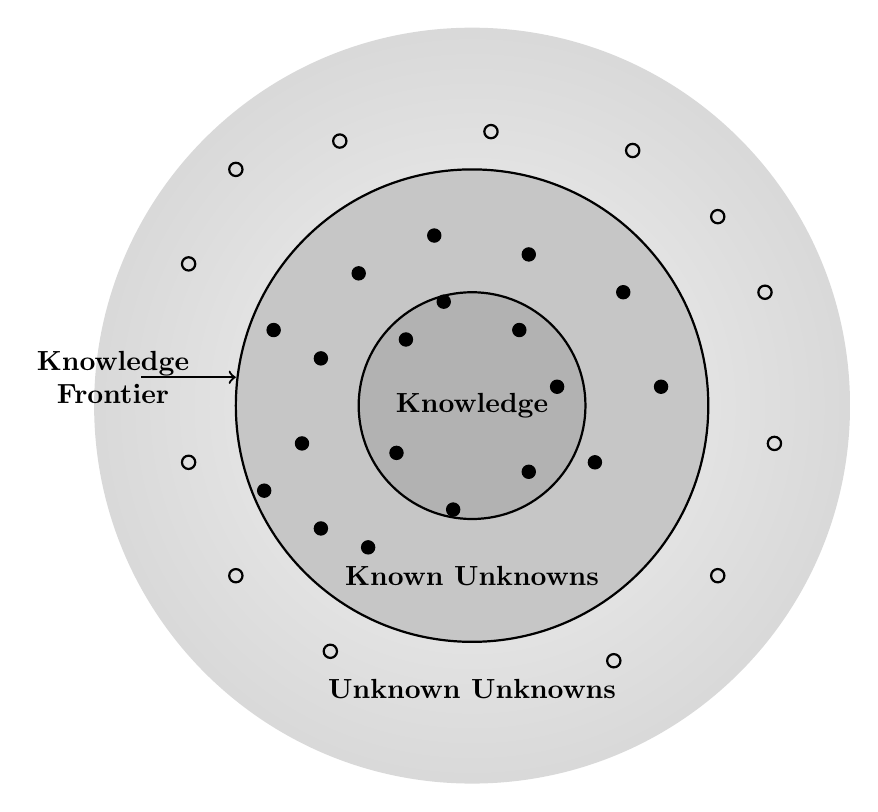
\begin{tikzpicture}[scale=1.2]

% Background gradient only (no border for outermost area)
\shade[inner color=gray!10, outer color=gray!30] (0,0) circle (4);

% Middle circle: Known Unknowns (with border)
\filldraw[fill=gray!45, draw=black, thick] (0,0) circle (2.5);
\node at (0,-3.0) {\textbf{Unknown Unknowns}};
\node at (0,-1.8) {\textbf{Known Unknowns}};

% Inner circle: Knowledge (with border)
\filldraw[fill=gray!60, draw=black, thick] (0,0) circle (1.2);
\node at (0,0) {\textbf{Knowledge}};

% Knowledge Frontier label
\node[align=center] at (-3.8,0.3) {\textbf{Knowledge} \\ \textbf{Frontier}};
\draw[->, thick] (-3.5,0.3) -- (-2.5,0.3);

% Known topics (solid dots)
\foreach \x/\y in {
  -0.7/0.7, -0.3/1.1, 0.5/0.8, 0.9/0.2, 0.6/-0.7, -0.2/-1.1, -0.8/-0.5,
  -1.6/0.5, -1.2/1.4, -0.4/1.8, 0.6/1.6, 1.6/1.2, 2/0.2, 1.3/-0.6,
  -1.1/-1.5, -1.8/-0.4, -2.1/0.8, -2.2/-0.9, -1.6/-1.3
}{
  \filldraw[black] (\x,\y) circle (2pt);
}

% Unknown unknowns (hollow circles)
\foreach \x/\y in {
  -3/1.5, -2.5/2.5, -1.4/2.8, 0.2/2.9, 1.7/2.7, 2.6/2, 3.1/1.2,
  3.2/-0.4, 2.6/-1.8, 1.5/-2.7, -1.5/-2.6, -2.5/-1.8, -3/-0.6
}{
  \draw[black, thick] (\x,\y) circle (2pt);
}

% Arrows pointing to new topics
% \draw[->, thick] (-0.4,1.8) -- (0.1,2.8);
% \draw[->, thick] (0.6,1.7) -- (0.3,2.8);
% \node at (0.2,3.4) {\text{New Research Topic}};

\end{tikzpicture}
\caption{\label{fig:NewTopics}The structure of knowledge.}
\end{figure}

%
% Section: References
%

\section*{References}

The theory of nescience builds upon several well-established foundations in information theory, computability, algorithmic complexity, and the philosophy of science. The following references provide the theoretical background and conceptual tools necessary to understand and situate the ideas introduced in this chapter.
 
Sipser's book \cite{sipser2012introduction} is a widely respected introduction to formal languages, automata, and computability theory. It lays the groundwork for understanding which descriptions are computationally feasible, an essential aspect of the theory of nescience, as it assumes that knowledge must be computable to be meaningful.

Li and Vitányi's book \cite{li2013introduction} is a comprehensive volume that presents the theory of Kolmogorov complexity, which formalizes the idea of description length using the shortest program capable of generating a given object. The concepts developed by Li and Vitányi are central to the theory of nescience, especially in defining metrics such as inaccuracy, miscoding, and surfeit based on algorithmic information theory.

Cover and Thomas's book \cite{cover2012elements} is a foundational text in information theory, providing the mathematical framework for understanding concepts such as entropy, mutual information, and data compression. It serves as a rigorous yet accessible introduction to how information can be quantified, transmitted, and encoded, ideas that relate to the notions of description length in the theory of nescience.

Chalmers's book \cite{chalmers2013thing} offers a critical and historical introduction to the philosophy of science. It examines the assumptions, limits, and methodologies of scientific practice. This perspective is invaluable for situating the theory of nescience within the broader discourse about how scientific knowledge is constructed, evaluated, and refined over time.
